\documentclass[11pt,a4paper]{article}

\usepackage[margin=1in]{geometry}
\usepackage{amsmath,amssymb}
\usepackage{graphicx}
\usepackage{float}
\usepackage{booktabs}
\usepackage{verbatim}
\usepackage{hyperref}
\usepackage{xcolor}
\usepackage{enumitem}

\graphicspath{{figures/}}

\hypersetup{
  colorlinks=true,
  linkcolor=black,
  urlcolor=blue
}

\setlength{\parindent}{0pt}
\setlength{\parskip}{0.7em}

\title{37495 Statistical Design and Models for Evaluation Studies\\
Assessment Task 2: R Assignment}
\author{Mario Rubiano\\Student ID: 24900627}
\date{}

\begin{document}
\maketitle

\begin{center}
\textbf{Submission file:} \texttt{37495\_Assignment\_Rubiano\_Mario}
\end{center}

This report includes the R code and the output that is used in the answers. The analysis uses the R functions and packages introduced in the laboratory solution files, including \texttt{aov}, \texttt{resid}, \texttt{shapiro.test}, \texttt{nortest::cvm.test}, \texttt{nortest::ad.test}, \texttt{lawstat::levene.test}, \texttt{MASS::boxcox}, \texttt{DescTools::BoxCox}, \texttt{emmeans}, \texttt{contrast} with Scheffe adjustment, \texttt{durbinWatsonTest}, and \texttt{cooks.distance}.

\section*{Question 1}

An appropriate design for this situation is a randomised complete block design. The response variable is the yield of the chemical process. This yield must be measured in the units used by the plant, for example grams, kilograms, or percent yield. The experimental factor is the chemical input, with five treatment levels because there are five chemicals. The blocking factor is technician, with three blocks because there are three technicians.

There are 15 experimental units in total. Each experimental unit is one individual execution of the chemical process by one specific technician using one specified chemical input. The measurement unit is the physical batch or final product sample where the yield is measured. Within each technician block, the five chemicals should be randomly allocated to the five process runs done by that technician. In this way, each chemical has three observations, and the design controls for differences between technicians.

A suitable model is
\[
y_{ij} = \mu + \tau_i + \beta_j + e_{ij},
\]
where $\tau_i$ is the effect of chemical $i$, $\beta_j$ is the effect of technician $j$, and $e_{ij}$ is the random error.

\section*{Question 2}

\subsection*{(a)}

For production run 1, the hypotheses are
\[
H_0: \mu_1 \leq 0.78,
\qquad
H_1: \mu_1 > 0.78.
\]

The sample mean is 0.831. The manual one-sample t-test gives $t = 1.67193$, $df = 19$, and $p = 0.05546308$. The 95 percent one-sided lower confidence bound is 0.7782551. Since $p > 0.05$, there is not enough evidence at the 5 percent level to conclude that the mean impact strength for production run 1 is greater than 0.78.

\begin{verbatim}
Manual one-sample t-test output:
mean = 0.831
t = 1.67193
df = 19
p-value = 0.05546308
95 percent one-sided lower confidence bound = 0.7782551
\end{verbatim}

\subsection*{(b)}

Using \texttt{set.seed(37495)}, 100000 bootstrap resamples of production run 1 gave a bootstrap mean distribution with mean approximately 0.8309 and standard deviation approximately 0.02986.

\begin{figure}[H]
\centering
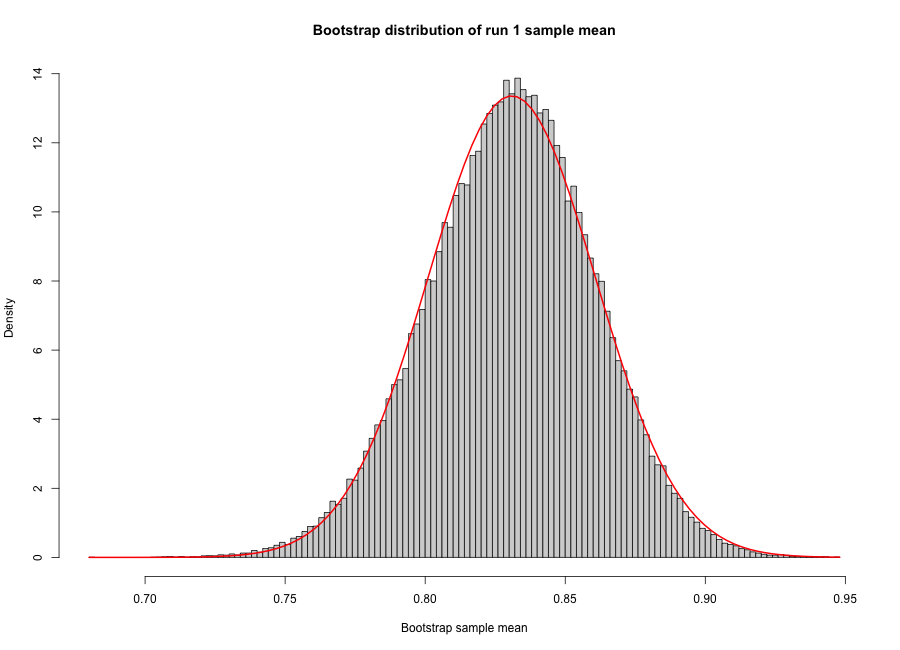
\includegraphics[width=0.85\textwidth]{q2b_bootstrap_histogram.png}
\caption{Bootstrap distribution of the run 1 sample mean with fitted normal density.}
\end{figure}

A Shapiro-Wilk test on a random sample of 50 bootstrap means gave $W = 0.96968$ and $p = 0.2246$. Since $p > 0.05$, the test does not show evidence against normality for the sampled bootstrap means. Together with the histogram, this suggests that the bootstrap distribution is approximately normal.

\begin{verbatim}
Bootstrap summary:
   Min. 1st Qu.  Median    Mean 3rd Qu.    Max.
 0.6805  0.8110  0.8315  0.8309  0.8510  0.9470

Shapiro-Wilk normality test
data:  sample(boot_means, 50)
W = 0.96968, p-value = 0.2246
\end{verbatim}

\subsection*{(c)}

For the ANOVA model \texttt{strength \textasciitilde run}, the ANOVA table is:

\begin{verbatim}
            Df Sum Sq Mean Sq F value Pr(>F)
run          4  2.791  0.6978   61.33 <2e-16 ***
Residuals   95  1.081  0.0114
\end{verbatim}

Since $p < 0.05$, the null hypothesis that all production run means are equal is rejected. This result shows strong evidence that the mean impact strength changes with production run.

\subsection*{(d)}

For the original ANOVA residuals, the normality tests were Shapiro-Wilk $W = 0.97714$, $p = 0.07935$, Cramer-von Mises $W = 0.058549$, $p = 0.3919$, and Anderson-Darling $A = 0.43981$, $p = 0.2865$. All three p-values are greater than 0.05, so normality is not rejected at the 5 percent level.

The modified Brown-Forsythe Levene test from \texttt{lawstat} gave test statistic 3.2344 and $p = 0.01579$, so the constant variance assumption is rejected at the 5 percent level.

\begin{verbatim}
Shapiro-Wilk normality test
data:  insulation$resid
W = 0.97714, p-value = 0.07935

Cramer-von Mises normality test
data:  insulation$resid
W = 0.058549, p-value = 0.3919

Anderson-Darling normality test
data:  insulation$resid
A = 0.43981, p-value = 0.2865

Modified robust Brown-Forsythe Levene-type test
data:  insulation$resid
Test Statistic = 3.2344, p-value = 0.01579
\end{verbatim}

\begin{figure}[H]
\centering
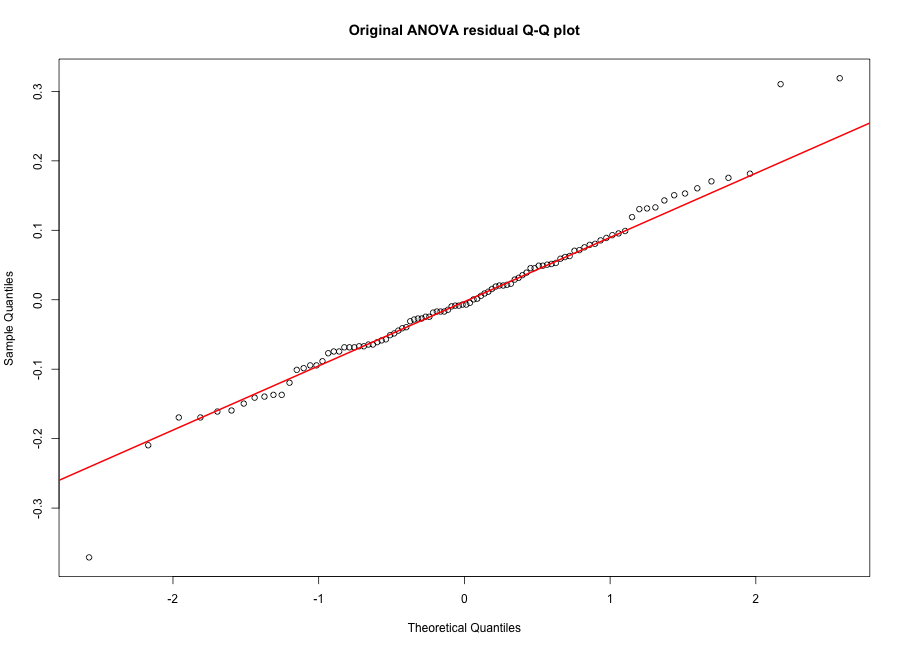
\includegraphics[width=0.78\textwidth]{q2d_original_residual_qq.png}
\caption{Q-Q plot for residuals from the original ANOVA model.}
\end{figure}

\begin{figure}[H]
\centering
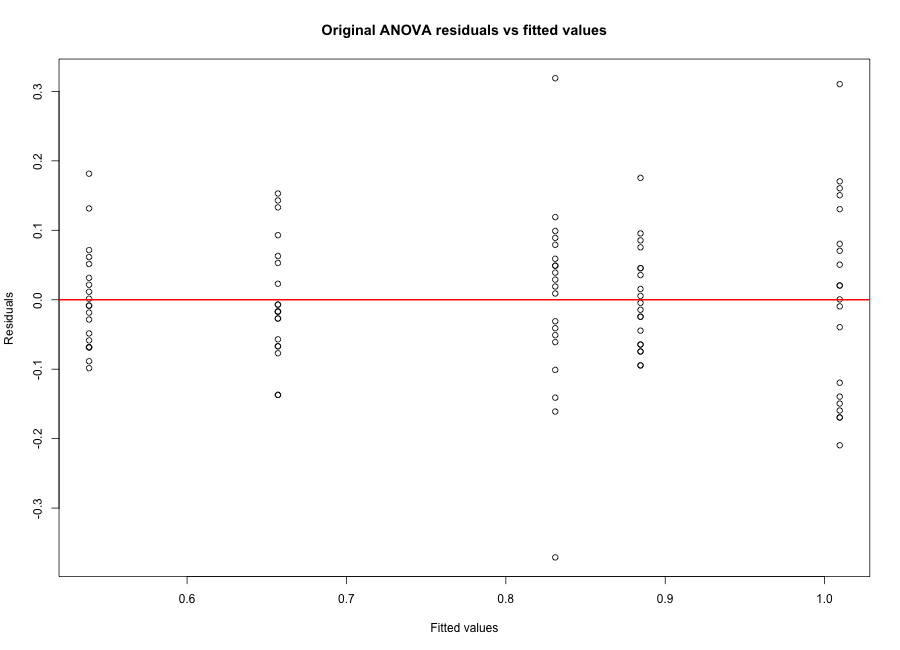
\includegraphics[width=0.78\textwidth]{q2d_original_residuals_vs_fitted.png}
\caption{Residuals versus fitted values for the original ANOVA model.}
\end{figure}

\subsection*{(e)}

Using \texttt{boxcox} from the \texttt{MASS} package, the optimal Box-Cox parameter was approximately
\[
\lambda = 0.245409.
\]

The transformed response used in the script is computed using \texttt{DescTools::BoxCox}:
\[
\texttt{strength\_bc = BoxCox(strength, lambda)}.
\]

\begin{figure}[H]
\centering
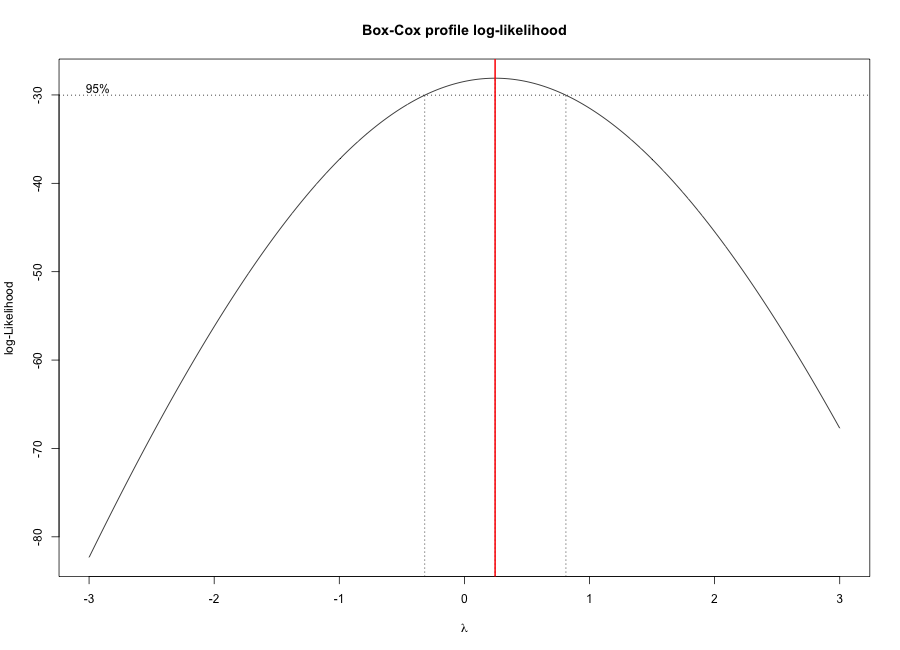
\includegraphics[width=0.85\textwidth]{q2e_boxcox_profile.png}
\caption{Box-Cox profile log-likelihood for the original ANOVA model.}
\end{figure}

\subsection*{(f)}

For the Box-Cox transformed ANOVA, the ANOVA table is:

\begin{verbatim}
            Df Sum Sq Mean Sq F value Pr(>F)
run          4  4.306  1.0765   66.75 <2e-16 ***
Residuals   95  1.532  0.0161
\end{verbatim}

For the transformed residuals, Shapiro-Wilk gave $W = 0.97188$, $p = 0.03082$, Cramer-von Mises gave $W = 0.030456$, $p = 0.8391$, and Anderson-Darling gave $A = 0.2938$, $p = 0.594$. Shapiro-Wilk rejects normality at the 5 percent level, but the Cramer-von Mises and Anderson-Darling tests do not reject it.

The modified Brown-Forsythe Levene test gave test statistic 1.3594 and $p = 0.2544$, so the constant variance assumption is not rejected after the transformation.

\begin{verbatim}
Shapiro-Wilk normality test
data:  insulation$resid_bc
W = 0.97188, p-value = 0.03082

Cramer-von Mises normality test
data:  insulation$resid_bc
W = 0.030456, p-value = 0.8391

Anderson-Darling normality test
data:  insulation$resid_bc
A = 0.2938, p-value = 0.594

Modified robust Brown-Forsythe Levene-type test
data:  insulation$resid_bc
Test Statistic = 1.3594, p-value = 0.2544
\end{verbatim}

\begin{figure}[H]
\centering
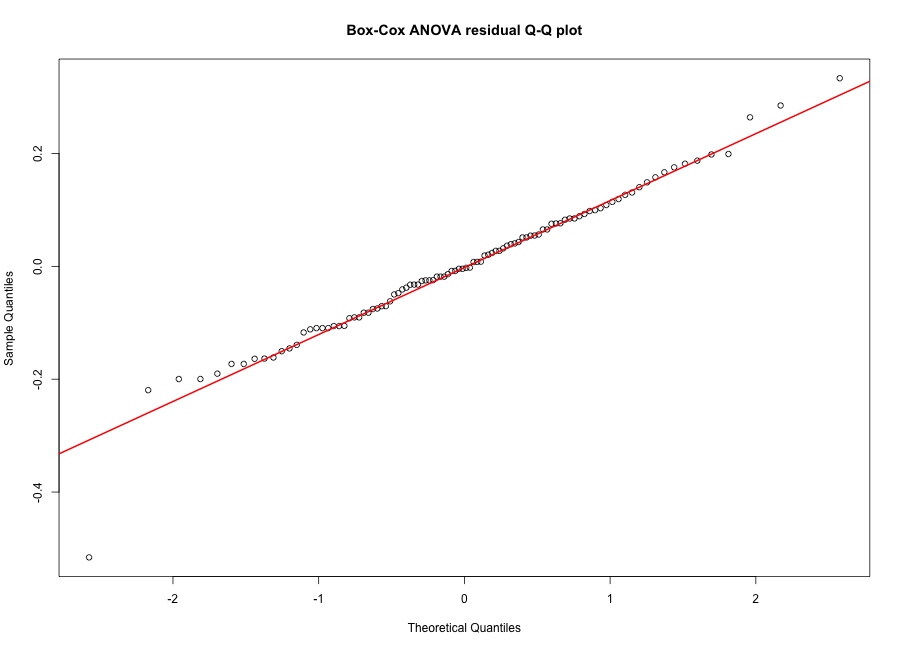
\includegraphics[width=0.78\textwidth]{q2f_boxcox_residual_qq.png}
\caption{Q-Q plot for residuals from the Box-Cox transformed ANOVA model.}
\end{figure}

\begin{figure}[H]
\centering
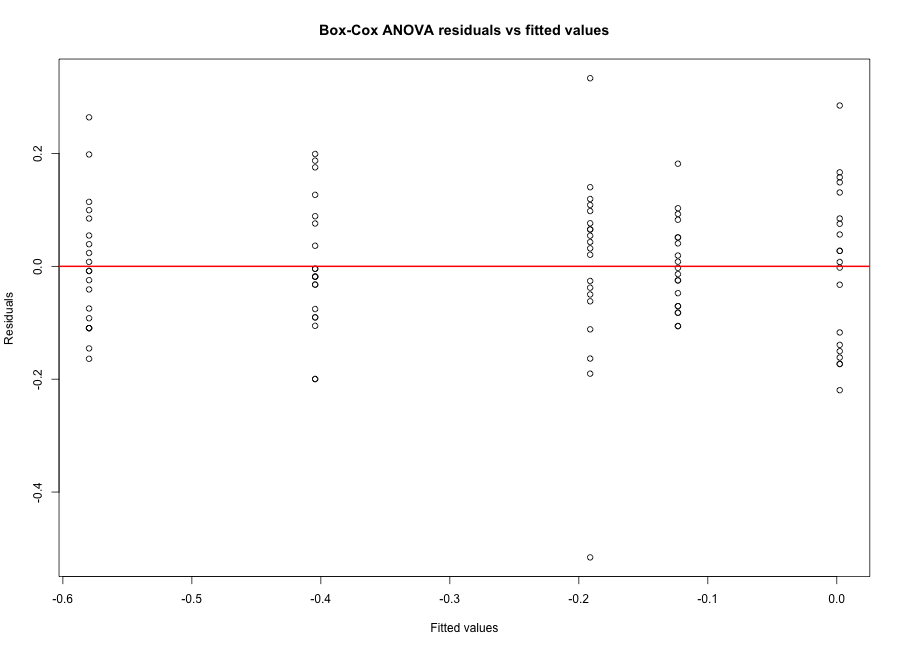
\includegraphics[width=0.78\textwidth]{q2f_boxcox_residuals_vs_fitted.png}
\caption{Residuals versus fitted values for the Box-Cox transformed ANOVA model.}
\end{figure}

\subsection*{(g)}

Using Scheffe adjustment through \texttt{emmeans}, the fitted contrasts on the Box-Cox transformed scale are:

\begin{verbatim}
contrast                estimate     SE df lower.CL upper.CL t.ratio p.value
run1_vs_avg_run2_5         0.085 0.0317 95 -0.00532    0.175   2.679  0.0734
run1_vs_run3               0.213 0.0402 95  0.09892    0.328   5.310 <0.0001
avg_run124_vs_avg_run35    0.388 0.0259 95  0.31425    0.462  14.969 <0.0001
\end{verbatim}

At the 5 percent level, contrast (i) is not significant. In contrast, contrasts (ii) and (iii) are significant.

\subsection*{(h)}

The Durbin-Watson test rejects the null hypothesis of no autocorrelation:

\begin{verbatim}
 lag Autocorrelation D-W Statistic p-value
   1       0.5695786     0.6416623       0
 Alternative hypothesis: rho != 0
\end{verbatim}

The apparent autocorrelation pattern occurs because the observations were entered in sorted order within each production run, and not in the random experimental order. In the data table, the 20 strength values for each run are listed from small to large before moving to the next run. This creates a clear pattern in the residuals when they are plotted by observation number. Therefore, the Durbin-Watson result is mainly responding to the artificial order in the table, not necessarily to real time-based autocorrelation in the process.

\subsection*{(i)}

The Cook's distance filtering rule \texttt{Cook's D <= 0.05} removes 3 observations, leaving 97 observations. The first 40 records of the filtered data set are:

\begin{verbatim}
 strength_bc run
 -0.38142711   1
 -0.35467008   1
 -0.30286466   1
 -0.25315901   1
 -0.24103808   1
 -0.22903385   1
 -0.21714374   1
 -0.17067592   1
 -0.15932067   1
 -0.14806578   1
 -0.13690923   1
 -0.12584902   1
 -0.12584902   1
 -0.11488325   1
 -0.09322766   1
 -0.08253430   1
 -0.07192829   1
 -0.05097181   1
 -0.21714374   2
 -0.17067592   2
 -0.17067592   2
 -0.15932067   2
 -0.14806578   2
 -0.13690923   2
 -0.11488325   2
 -0.03034565   2
  0.00000000   2
  0.00996249   2
  0.02966627   2
  0.02966627   2
  0.05868752   2
  0.07769242   2
  0.08709543   2
  0.13315767   2
  0.15115612   2
  0.16006766   2
  0.16892191   2
 -0.60415333   3
 -0.60415333   3
 -0.50988698   3
\end{verbatim}

The removed observations were:

\begin{verbatim}
   run strength strength_bc     cooksD
1    1     0.46  -0.7070227 0.18279886
20   1     1.15   0.1421864 0.07637505
40   2     1.32   0.2873082 0.05582352
\end{verbatim}

\section*{Question 3}

The model is
\[
y_{ij}= \mu + \tau_i + e_{ij}, \qquad i=1,\ldots,a,\quad j=1,\ldots,n,
\]
with constraint
\[
\sum_{i=1}^a \tau_i = 0.
\]

The least squares criterion is
\[
S(\mu,\tau)=\sum_{i=1}^a\sum_{j=1}^n (y_{ij}-\mu-\tau_i)^2.
\]

Using a Lagrange multiplier for the constraint, minimise
\[
L = \sum_{i=1}^a\sum_{j=1}^n (y_{ij}-\mu-\tau_i)^2
    + 2\gamma\sum_{i=1}^a \tau_i.
\]

Differentiating with respect to $\mu$ gives
\[
-2\sum_{i=1}^a\sum_{j=1}^n (y_{ij}-\mu-\tau_i)=0.
\]
Therefore,
\[
\sum_{i=1}^a\sum_{j=1}^n y_{ij}=an\mu+n\sum_{i=1}^a\tau_i.
\]
Since $\sum_i \tau_i = 0$,
\[
\hat{\mu}=\bar{y}_{..}.
\]

Differentiating with respect to $\tau_i$ gives
\[
-2\sum_{j=1}^n (y_{ij}-\mu-\tau_i)+2\gamma=0,
\]
so
\[
\sum_{j=1}^n y_{ij}-n\mu-n\tau_i=\gamma.
\]
Summing this equation over $i$ gives
\[
\sum_{i=1}^a\sum_{j=1}^n y_{ij}-an\mu-n\sum_{i=1}^a\tau_i = a\gamma.
\]
Using $\hat{\mu}=\bar{y}_{..}$ and $\sum_i \tau_i=0$, the left side is zero, hence $\gamma=0$. Therefore,
\[
n\bar{y}_{i.}-n\mu-n\tau_i=0,
\]
and
\[
\hat{\tau}_i=\bar{y}_{i.}-\bar{y}_{..}.
\]

The fitted value is
\[
\hat{y}_{ij}=\hat{\mu}+\hat{\tau}_i=\bar{y}_{i.}.
\]
Therefore the residual is
\[
\hat{e}_{ij}=y_{ij}-\bar{y}_{i.}.
\]

Because $\bar{y}_{i.}$ is the mean of the $n$ observations in treatment $i$,
\[
\operatorname{Var}(\hat{e}_{ij})
= \operatorname{Var}(y_{ij}-\bar{y}_{i.})
= \operatorname{Var}(y_{ij})+\operatorname{Var}(\bar{y}_{i.})
-2\operatorname{Cov}(y_{ij},\bar{y}_{i.}).
\]

Now,
\[
\operatorname{Var}(y_{ij})=\sigma^2,\qquad
\operatorname{Var}(\bar{y}_{i.})=\frac{\sigma^2}{n},
\]
and
\[
\operatorname{Cov}(y_{ij},\bar{y}_{i.})
=\operatorname{Cov}\left(y_{ij},\frac{1}{n}\sum_{k=1}^n y_{ik}\right)
=\frac{\sigma^2}{n},
\]
since only the term with $k=j$ contributes to the covariance. Hence,
\[
\operatorname{Var}(\hat{e}_{ij})
= \sigma^2+\frac{\sigma^2}{n}-2\frac{\sigma^2}{n}
= \sigma^2\left(1-\frac{1}{n}\right).
\]

\newpage
\appendix
\section*{Appendix: R code used for the analysis}

\verbatiminput{assignment_solution.R}

\end{document}
